\documentclass[11pt]{article}
\usepackage{microtype}
\usepackage{graphicx}
\usepackage{wrapfig}
\usepackage{url}
\usepackage{wrapfig}
\usepackage{color}
\usepackage{marvosym}
\usepackage{enumerate}
\usepackage{subfigure}
\usepackage{tikz}
\usepackage[fleqn]{amsmath}
\DeclareMathOperator*{\argmax}{arg\,max}
\DeclareMathOperator*{\argmin}{arg\,min}
\usepackage{amssymb}
\usepackage{hyperref}
\usepackage[many]{tcolorbox}
\usepackage{lipsum}
\usepackage{float}
\usepackage{trimclip}
\usepackage{listings}
\usepackage{environ}% http://ctan.org/pkg/environ
\usepackage{wasysym}
\usepackage{array}

\def\ci{\perp\!\!\!\perp}

\oddsidemargin 0mm
\evensidemargin 5mm
\topmargin -20mm
\textheight 240mm
\textwidth 160mm

\newcommand{\vwi}{{\bf w}_i}
\newcommand{\vw}{{\bf w}}
\newcommand{\vx}{{\bf x}}
\newcommand{\vy}{{\bf y}}
\newcommand{\vxi}{{\bf x}_i}
\newcommand{\yi}{y_i}
\newcommand{\vxj}{{\bf x}_j}
\newcommand{\vxn}{{\bf x}_n}
\newcommand{\yj}{y_j}
\newcommand{\ai}{\alpha_i}
\newcommand{\aj}{\alpha_j}
\newcommand{\X}{{\bf X}}
\newcommand{\Y}{{\bf Y}}
\newcommand{\vz}{{\bf z}}
\newcommand{\msigma}{{\bf \Sigma}}
\newcommand{\vmu}{{\bf \mu}}
\newcommand{\vmuk}{{\bf \mu}_k}
\newcommand{\msigmak}{{\bf \Sigma}_k}
\newcommand{\vmuj}{{\bf \mu}_j}
\newcommand{\msigmaj}{{\bf \Sigma}_j}
\newcommand{\pij}{\pi_j}
\newcommand{\pik}{\pi_k}
\newcommand{\D}{\mathcal{D}}
\newcommand{\el}{\mathcal{L}}
\newcommand{\N}{\mathcal{N}}
\newcommand{\vxij}{{\bf x}_{ij}}
\newcommand{\vt}{{\bf t}}
\newcommand{\yh}{\hat{y}}
\newcommand{\code}[1]{{\footnotesize \tt #1}}
\newcommand{\alphai}{\alpha_i}
\newcommand{\defeq}{\overset{\text{def}}{=}}
\renewcommand{\vec}[1]{\mathbf{#1}}


\bgroup
\def\arraystretch{1.5}
\newcolumntype{x}[1]{>{\centering\arraybackslash\hspace{0pt}}p{#1}}
\newcolumntype{z}[1]{>{\centering\arraybackslash}m{#1}}

%Arguments are 1 - height, 2 - box title
\newtcolorbox{textanswerbox}[2]{%
 width=\textwidth,colback=white,colframe=blue!30!black,floatplacement=H,height=#1,title=#2,clip lower=true,before upper={\parindent0em}}

 \newtcolorbox{eqanswerbox}[1]{%
 width=#1,colback=white,colframe=black,floatplacement=H,height=3em,sharp corners=all,clip lower=true,before upper={\parindent0em}}

 %Arguments are 1 - height, 2 - box title
 \NewEnviron{answertext}[2]{
        \noindent
        \marginbox*{0pt 10pt}{
        \clipbox{0pt 0pt 0pt 0pt}{
        \begin{textanswerbox}{#1}{#2}
        \BODY
        \end{textanswerbox}
        }
        }
}

%Arguments are 1 - height, 2 - box title, 3 - column definition
 \NewEnviron{answertable}[3]{
        \noindent
        \marginbox*{0pt 10pt}{
        \clipbox{0pt 0pt 0pt 0pt}{
        \begin{textanswerbox}{#1}{#2}
                \vspace{-0.5cm}
                        \begin{table}[H]
                        \centering
                        \begin{tabular}{#3}
                                \BODY
                        \end{tabular}
                        \end{table}
        \end{textanswerbox}
        }
        }
}

 %Arguments are 1 - height, 2 - box title, 3 - title, 4- equation label, 5 - equation box width
 \NewEnviron{answerequation}[5]{
        \noindent
        \marginbox*{0pt 10pt}{
        \clipbox{0pt 0pt 0pt 0pt}{
        \begin{textanswerbox}{#1}{#2}
                \vspace{-0.5cm}
                        \begin{table}[H]
                        \centering
                \renewcommand{\arraystretch}{0.5}% Tighter

                        \begin{tabular}{#3}
                                #4 =	&
                        \clipbox{0pt 0pt 0pt 0pt}{

                        \begin{eqanswerbox}{#5}
                                $\BODY$
                        \end{eqanswerbox}
                        } \\
                        \end{tabular}
                        \end{table}

        \end{textanswerbox}
        }
        }
}

 %Arguments are 1 - height, 2 - box title
 \NewEnviron{answerderivation}[2]{
        \noindent
        \marginbox*{0pt 10pt}{
        \clipbox{0pt 0pt 0pt 0pt}{
        \begin{textanswerbox}{#1}{#2}
        \BODY
        \end{textanswerbox}
        }
        }
}

\newcommand{\Checked}{{\LARGE \XBox}}%
\newcommand{\Unchecked}{{\LARGE \Square}}%
\newcommand{\TextRequired}{{\textbf{Place Answer Here}}}%
\newcommand{\EquationRequired}{\textbf{Type Equation Here}}%

\usetikzlibrary{shapes, arrows, calc, positioning,matrix}
\tikzset{
data/.style={circle, draw, text centered, minimum height=3em ,minimum width = .5em, inner sep = 2pt},
empty/.style={circle, text centered, minimum height=3em ,minimum width = .5em, inner sep = 2pt},
}
\newcommand{\ztnodesize}{.6}
\newcommand{\factorsize}{1}
\newcommand{\nodesize}{1.3}

\newcommand{\answertextheight}{5cm}
\newcommand{\answertableheight}{4cm}
\newcommand{\answerequationheight}{2.5cm}
\newcommand{\answerderivationheight}{14cm}

\newcounter{QuestionCounter}
\newcounter{SubQuestionCounter}[QuestionCounter]
\setcounter{SubQuestionCounter}{1}

\newcommand{\subquestiontitle}{Question \theQuestionCounter.\theSubQuestionCounter~}
\newcommand{\newquestion}{\stepcounter{QuestionCounter}\setcounter{SubQuestionCounter}{1}\newpage}
\newcommand{\newsubquestion}{\stepcounter{SubQuestionCounter}}

\DeclareMathOperator{\rank}{rank}
\DeclareMathOperator{\indices}{indices}
\DeclareMathOperator{\Bernoulli}{Bernoulli}
\DeclareMathOperator{\Bin}{Bin}
\DeclareMathOperator{\E}{E}
\DeclareMathOperator{\Var}{Var}
\DeclareMathOperator{\Cov}{Cov}

\lstset{language=[LaTeX]TeX,basicstyle=\ttfamily\bf}

\pagestyle{myheadings}
\markboth{Homework 5}{Fall 2021 CS 475/675 Machine Learning: Homework 5}

\title{CS 475 Machine Learning: Homework 5 Analytical \\
(70 points)\\
\Large{Assigned: Tuesday, Nov. 16th, 2021} \\
\Large{Due: Tuesday, Nov. 30th, 2021, 11:59 pm US/Eastern}}
\author{Partner 1: NAME (JHED), Partner 2:  NAME (JHED)}
\date{}

\begin{document}
\maketitle
\thispagestyle{headings}

\section*{Instructions }
We have provided this \LaTeX{} document for turning in this homework. We give you one or more boxes to answer each question.  The question to answer for each box will be noted in the title of the box.  You can change the size of the box if you need more space.\\

{\bf Other than your name, do not type anything outside the boxes. Leave the rest of the document unchanged.}\\


\textbf{
%Do not change any formatting in this document, or we may be unable to
  %grade your work. This includes, but is not limited to, the height of
  %textboxes, font sizes, and the spacing of text and tables.  Additionally,
  Do
  not add text outside of the answer boxes.  You are allowed to make boxes larger if needed.
  % Entering your answers are the only
  %changes allowed.
  }\\


\textbf{We strongly recommend you review your answers in the generated PDF to
  ensure they appear correct. We will grade what appears in the answer boxes in
  the submitted PDF, NOT the original latex file.}

% -----------------------------------------------------------

\pagebreak
\section*{Observational Equivalence of DAGs and the GES Algorithm}

{\bf Question 1.}

Two DAGs ${\cal G}_1$ and ${\cal G}_2$ are said to be \emph{observationally equivalent} if the list of conditional independences implied by the d-separation criterion in both graphs is the same.  In other words, ${\cal G}_1$ and ${\cal G}_2$ are observationally equivalent if they imply the same statistical model.

A result by Thomas Verma and Judea Pearl states that ${\cal G}_1$ and ${\cal G}_2$ are observationally equivalent if and only if they agree on edge adjacencies (in other words, if $V_i$ and $V_j$ share an edge in ${\cal G}_1$, then $V_i$ and $V_j$ share an edge in ${\cal G}_2$, and vice versa -- ignoring edge orientation), and agree on unshielded colliders.  An unshielded collider is a structure of the form $V_i \to V_k \gets V_j$ such that $V_i$ and $V_j$ do not share an edge.  As an example, the following three graphs are observationally equivalent:

\begin{center}
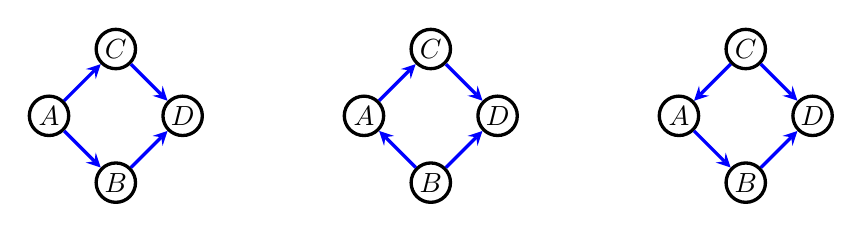
\begin{tikzpicture}[>=stealth, node distance=1.2cm]
    \tikzstyle{format} = [draw, very thick, circle, minimum size=5.0mm,
	inner sep=0pt]

	\begin{scope}
		\path[->, very thick]
			node[format] (1) {$A$}
			node[format, below right of=1] (2) {$B$}
			node[format, above right of=2] (4) {$D$}
			node[format, above left of=4] (3) {$C$}

			(1) edge[blue] (2)
			(1) edge[blue] (3)
			(2) edge[blue] (4)
			(3) edge[blue] (4)
		;
	\end{scope}
	\begin{scope}[xshift=4.0cm]
		\path[->, very thick]
			node[format] (1) {$A$}
			node[format, below right of=1] (2) {$B$}
			node[format, above right of=2] (4) {$D$}
			node[format, above left of=4] (3) {$C$}

			(2) edge[blue] (1)
			(1) edge[blue] (3)
			(2) edge[blue] (4)
			(3) edge[blue] (4)
		;
	\end{scope}
	\begin{scope}[xshift=8.0cm]
		\path[->, very thick]
			node[format] (1) {$A$}
			node[format, below right of=1] (2) {$B$}
			node[format, above right of=2] (4) {$D$}
			node[format, above left of=4] (3) {$C$}

			(1) edge[blue] (2)
			(3) edge[blue] (1)
			(2) edge[blue] (4)
			(3) edge[blue] (4)
		;
	\end{scope}
\end{tikzpicture}
\end{center}
The above three DAGs give the same model: $(B \ci C \mid A)$, $(D \ci A \mid B,C)$.

\begin{enumerate}
\item[(a)] Write out all equivalence classes for DAGs with three vertices.  How many equivalence classes are there?
\item[(b)] Assume all data is binary.  Write down the dimension of each model corresponding to each equivalence class in (a).
\item[(c)] Create an undirected graph representing the discrete state space for structure learning, where vertices represent equivalence classes in (a), and there is an edge connecting any two classes where a DAG in one class differs from a DAG in another class by \emph{addition or deletion} precisely one $\to$ edge.
\item[(d)] 
Assume the GES algorithm performs the following sequence of edge additions and deletions (starting from the empty graph): add $A\to B$, add $B \to C$, add $A \to C$, remove $B \to C$.
Write down all sequences of equivalence classes consistent with this set of edge additions and removals.  Note: there could be more than one such sequence.

\item[(e)] Consider a DAG $V_1 \to V_2 \to V_3 \to V_4 \to V_k$.  How many DAGs are observationally equivalent to this DAG?  Explain.
\end{enumerate}

\begin{answertext}{22cm}{}
\begin{enumerate}

\item[(a)]
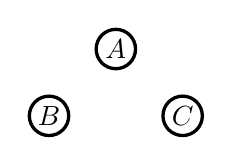
\begin{tikzpicture}[>=stealth, node distance=1.2cm]
	\tikzstyle{format} = [draw, very thick, circle, minimum size=5.0mm, inner sep=0pt]

	\begin{scope}
		\path[->, very thick]
			node[format] (1) {$A$}
			node[format, below left of=1] (2) {$B$}
			node[format, below right of=1] (3) {$C$}
		;
	\end{scope}
\end{tikzpicture} \\

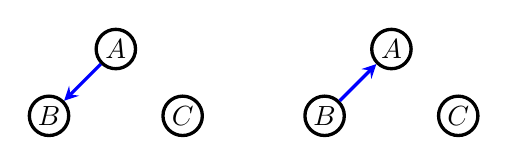
\begin{tikzpicture}[>=stealth, node distance=1.2cm]
	\tikzstyle{format} = [draw, very thick, circle, minimum size=5.0mm, inner sep=0pt]

	\begin{scope}
		\path[->, very thick]
			node[format] (1) {$A$}
			node[format, below left of=1] (2) {$B$}
			node[format, below right of=1] (3) {$C$}

			(1) edge[blue] (2)
		;
	\end{scope}

	\begin{scope}[xshift=3.5cm]
		\path[->, very thick]
			node[format] (1) {$A$}
			node[format, below left of=1] (2) {$B$}
			node[format, below right of=1] (3) {$C$}

			(2) edge[blue] (1)
		;
	\end{scope}
\end{tikzpicture} \\

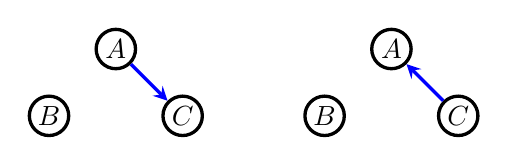
\begin{tikzpicture}[>=stealth, node distance=1.2cm]
	\tikzstyle{format} = [draw, very thick, circle, minimum size=5.0mm, inner sep=0pt]	

	\begin{scope}
		\path[->, very thick]
			node[format] (1) {$A$}
			node[format, below left of=1] (2) {$B$}
			node[format, below right of=1] (3) {$C$}

			(1) edge[blue] (3)
		;
	\end{scope}

	\begin{scope}[xshift=3.5cm]
		\path[->, very thick]
			node[format] (1) {$A$}
			node[format, below left of=1] (2) {$B$}
			node[format, below right of=1] (3) {$C$}

			(3) edge[blue] (1)
		;
	\end{scope}
\end{tikzpicture} \\

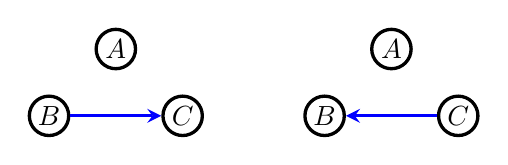
\begin{tikzpicture}[>=stealth, node distance=1.2cm]
	\tikzstyle{format} = [draw, very thick, circle, minimum size=5.0mm, inner sep=0pt]	

	\begin{scope}
		\path[->, very thick]
			node[format] (1) {$A$}
			node[format, below left of=1] (2) {$B$}
			node[format, below right of=1] (3) {$C$}

			(2) edge[blue] (3)
		;
	\end{scope}

	\begin{scope}[xshift=3.5cm]
		\path[->, very thick]
			node[format] (1) {$A$}
			node[format, below left of=1] (2) {$B$}
			node[format, below right of=1] (3) {$C$}

			(3) edge[blue] (2)
		;
	\end{scope}
\end{tikzpicture} \\

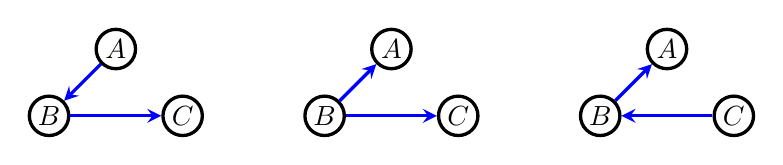
\begin{tikzpicture}[>=stealth, node distance=1.2cm]
	\tikzstyle{format} = [draw, very thick, circle, minimum size=5.0mm, inner sep=0pt]

	\begin{scope}
		\path[->, very thick]
			node[format] (1) {$A$}
			node[format, below left of=1] (2) {$B$}
			node[format, below right of=1] (3) {$C$}

			(1) edge[blue] (2)
			(2) edge[blue] (3)
		;
	\end{scope}

	\begin{scope}[xshift=3.5cm]
		\path[->, very thick]
			node[format] (1) {$A$}
			node[format, below left of=1] (2) {$B$}
			node[format, below right of=1] (3) {$C$}

			(2) edge[blue] (1)
			(2) edge[blue] (3)
		;
	\end{scope}

	\begin{scope}[xshift=7.0cm]
		\path[->, very thick]
			node[format] (1) {$A$}
			node[format, below left of=1] (2) {$B$}
			node[format, below right of=1] (3) {$C$}

			(2) edge[blue] (1)
			(3) edge[blue] (2)
		;
	\end{scope}
\end{tikzpicture} \\

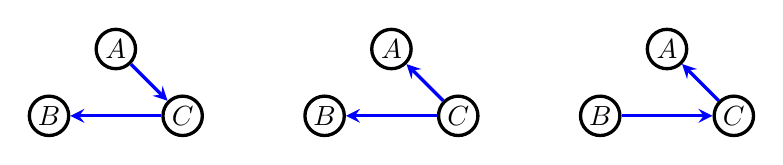
\begin{tikzpicture}[>=stealth, node distance=1.2cm]
	\tikzstyle{format} = [draw, very thick, circle, minimum size=5.0mm, inner sep=0pt]

	\begin{scope}
		\path[->, very thick]
			node[format] (1) {$A$}
			node[format, below left of=1] (2) {$B$}
			node[format, below right of=1] (3) {$C$}

			(1) edge[blue] (3)
			(3) edge[blue] (2)
		;
	\end{scope}		

	\begin{scope}[xshift=3.5cm]
		\path[->, very thick]
			node[format] (1) {$A$}
			node[format, below left of=1] (2) {$B$}
			node[format, below right of=1] (3) {$C$}

			(3) edge[blue] (1)
			(3) edge[blue] (2)
		;
	\end{scope}		

	\begin{scope}[xshift=7.0cm]
		\path[->, very thick]
			node[format] (1) {$A$}
			node[format, below left of=1] (2) {$B$}
			node[format, below right of=1] (3) {$C$}

			(3) edge[blue] (1)
			(2) edge[blue] (3)
		;
	\end{scope}		
\end{tikzpicture} \\

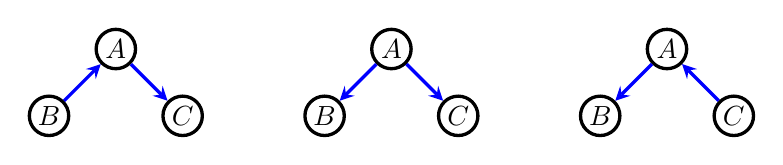
\begin{tikzpicture}[>=stealth, node distance=1.2cm]
	\tikzstyle{format} = [draw, very thick, circle, minimum size=5.0mm, inner sep=0pt]

	\begin{scope}
		\path[->, very thick]
			node[format] (1) {$A$}
			node[format, below left of=1] (2) {$B$}
			node[format, below right of=1] (3) {$C$}

			(2) edge[blue] (1)
			(1) edge[blue] (3)
		;
	\end{scope}

	\begin{scope}[xshift=3.5cm]
		\path[->, very thick]
			node[format] (1) {$A$}
			node[format, below left of=1] (2) {$B$}
			node[format, below right of=1] (3) {$C$}

			(1) edge[blue] (2)
			(1) edge[blue] (3)
		;
	\end{scope}

	\begin{scope}[xshift=7.0cm]
		\path[->, very thick]
			node[format] (1) {$A$}
			node[format, below left of=1] (2) {$B$}
			node[format, below right of=1] (3) {$C$}

			(1) edge[blue] (2)
			(3) edge[blue] (1)
		;
	\end{scope}
\end{tikzpicture} \\

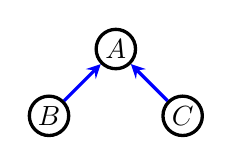
\begin{tikzpicture}[>=stealth, node distance=1.2cm]
	\tikzstyle{format} = [draw, very thick, circle, minimum size=5.0mm, inner sep=0pt]

	\begin{scope}
		\path[->, very thick]
			node[format] (1) {$A$}
			node[format, below left of=1] (2) {$B$}
			node[format, below right of=1] (3) {$C$}

			(2) edge[blue] (1)
			(3) edge[blue] (1)
		;
	\end{scope}
\end{tikzpicture} \\

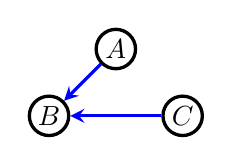
\begin{tikzpicture}[>=stealth, node distance=1.2cm]
	\tikzstyle{format} = [draw, very thick, circle, minimum size=5.0mm, inner sep=0pt]

	\begin{scope}[xshift=3.5cm]
		\path[->, very thick]
			node[format] (1) {$A$}
			node[format, below left of=1] (2) {$B$}
			node[format, below right of=1] (3) {$C$}

			(1) edge[blue] (2)
			(3) edge[blue] (2)
		;
	\end{scope}		
\end{tikzpicture} \\

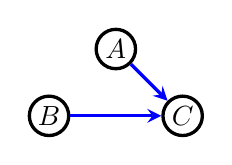
\begin{tikzpicture}[>=stealth, node distance=1.2cm]
	\tikzstyle{format} = [draw, very thick, circle, minimum size=5.0mm, inner sep=0pt]

	\begin{scope}[xshift=7.0cm]
		\path[->, very thick]
			node[format] (1) {$A$}
			node[format, below left of=1] (2) {$B$}
			node[format, below right of=1] (3) {$C$}

			(1) edge[blue] (3)
			(2) edge[blue] (3)
		;
	\end{scope}
\end{tikzpicture} \\

\end{enumerate}
\end{answertext}

\begin{answertext}{22cm}{}
\begin{enumerate}
\item[]
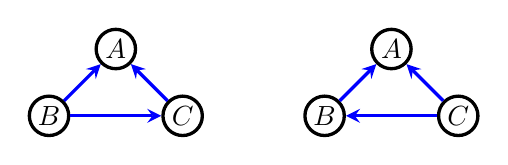
\begin{tikzpicture}[>=stealth, node distance=1.2cm]
	\tikzstyle{format} = [draw, very thick, circle, minimum size=5.0mm, inner sep=0pt]

	\begin{scope}
		\path[->, very thick]
			node[format] (1) {$A$}
			node[format, below left of=1] (2) {$B$}
			node[format, below right of=1] (3) {$C$}

			(2) edge[blue] (1)
			(3) edge[blue] (1)
			(2) edge[blue] (3)
		;
	\end{scope}

	\begin{scope}[xshift=3.5cm]
		\path[->, very thick]
			node[format] (1) {$A$}
			node[format, below left of=1] (2) {$B$}
			node[format, below right of=1] (3) {$C$}

			(2) edge[blue] (1)
			(3) edge[blue] (1)
			(3) edge[blue] (2)
		;
	\end{scope}
\end{tikzpicture} \\

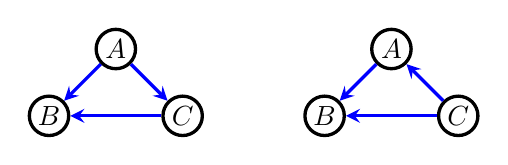
\begin{tikzpicture}[>=stealth, node distance=1.2cm]
	\tikzstyle{format} = [draw, very thick, circle, minimum size=5.0mm, inner sep=0pt]

	\begin{scope}
		\path[->, very thick]
			node[format] (1) {$A$}
			node[format, below left of=1] (2) {$B$}
			node[format, below right of=1] (3) {$C$}

			(1) edge[blue] (2)
			(3) edge[blue] (2)
			(1) edge[blue] (3)
		;
	\end{scope}

	\begin{scope}[xshift=3.5cm]
		\path[->, very thick]
			node[format] (1) {$A$}
			node[format, below left of=1] (2) {$B$}
			node[format, below right of=1] (3) {$C$}

			(1) edge[blue] (2)
			(3) edge[blue] (2)
			(3) edge[blue] (1)
		;
	\end{scope}		
\end{tikzpicture} \\

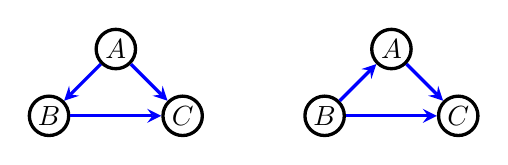
\begin{tikzpicture}[>=stealth, node distance=1.2cm]
	\tikzstyle{format} = [draw, very thick, circle, minimum size=5.0mm, inner sep=0pt]

	\begin{scope}
		\path[->, very thick]
			node[format] (1) {$A$}
			node[format, below left of=1] (2) {$B$}
			node[format, below right of=1] (3) {$C$}

			(1) edge[blue] (3)
			(2) edge[blue] (3)
			(1) edge[blue] (2)
		;
	\end{scope}

	\begin{scope}[xshift=3.5cm]
		\path[->, very thick]
			node[format] (1) {$A$}
			node[format, below left of=1] (2) {$B$}
			node[format, below right of=1] (3) {$C$}

			(1) edge[blue] (3)
			(2) edge[blue] (3)
			(2) edge[blue] (1)
		;
	\end{scope}
\end{tikzpicture} \\

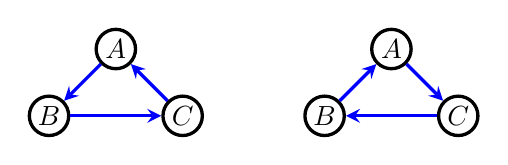
\begin{tikzpicture}[>=stealth, node distance=1.2cm]
	\tikzstyle{format} = [draw, very thick, circle, minimum size=5.0mm, inner sep=0pt]

	\begin{scope}
		\path[->, very thick]
			node[format] (1) {$A$}
			node[format, below left of=1] (2) {$B$}
			node[format, below right of=1] (3) {$C$}

			(1) edge[blue] (2)
			(2) edge[blue] (3)
			(3) edge[blue] (1)
		;
	\end{scope}

	\begin{scope}[xshift=3.5cm]
		\path[->, very thick]
			node[format] (1) {$A$}
			node[format, below left of=1] (2) {$B$}
			node[format, below right of=1] (3) {$C$}

			(2) edge[blue] (1)
			(3) edge[blue] (2)
			(1) edge[blue] (3)
		;
	\end{scope}
\end{tikzpicture} \\
Each line represents all DAGs in an equivalent class. There are a total of 14 equivalent classes. \\

\item[(b)]
We order the classes in (a) with number 1 - 14 in the order that they are listed. \\
\begin{enumerate}
\item[case 1:]
$p = p(A)p(B)p(C)$ \\
dimension: $1 + 1 + 1 = 3$
\item[case 2:]
$p = p(A)p(B \mid A)p(C)$ \\
dimension: $1 + 2 + 1 = 4$
\item[case 3:]
Similar to case 2, dimension: $4$
\item[case 4:]
Similar to case 2, dimension: $4$
\item[case 5:]
$p = p(A)p(B \mid A)p(C \mid B)$
dimension: $1 + 2 + 2 = 5$
\item[case 6:]
Similar to case 5, dimension: $5$
\item[case 7:]
Similar to case 5, dimension: $5$
\item[case 8:]
$p = p(B)p(C)p(A \mid B,C)$
dimension: $1 + 1 + 4 = 6$
\item[case 9:]
Similar to case 8, dimension: $6$
\item[case 10:]
Similar to case 8, dimension: $6$
\item[case 11:]
$p = p(B)p(C \mid B)p(A \mid B,C)$
dimension: $1 + 2 + 4 = 7$
\item[case 12:]
Similar to case 11, dimension: $7$
\item[case 13:]
Similar to case 11, dimension: $7$
\item[case 14:]
$p = p(A,B,C)$
dimension: $7$
\end{enumerate}
\end{enumerate}
\end{answertext}

\begin{answertext}{22cm}{}
\begin{enumerate}
\item[(c)]
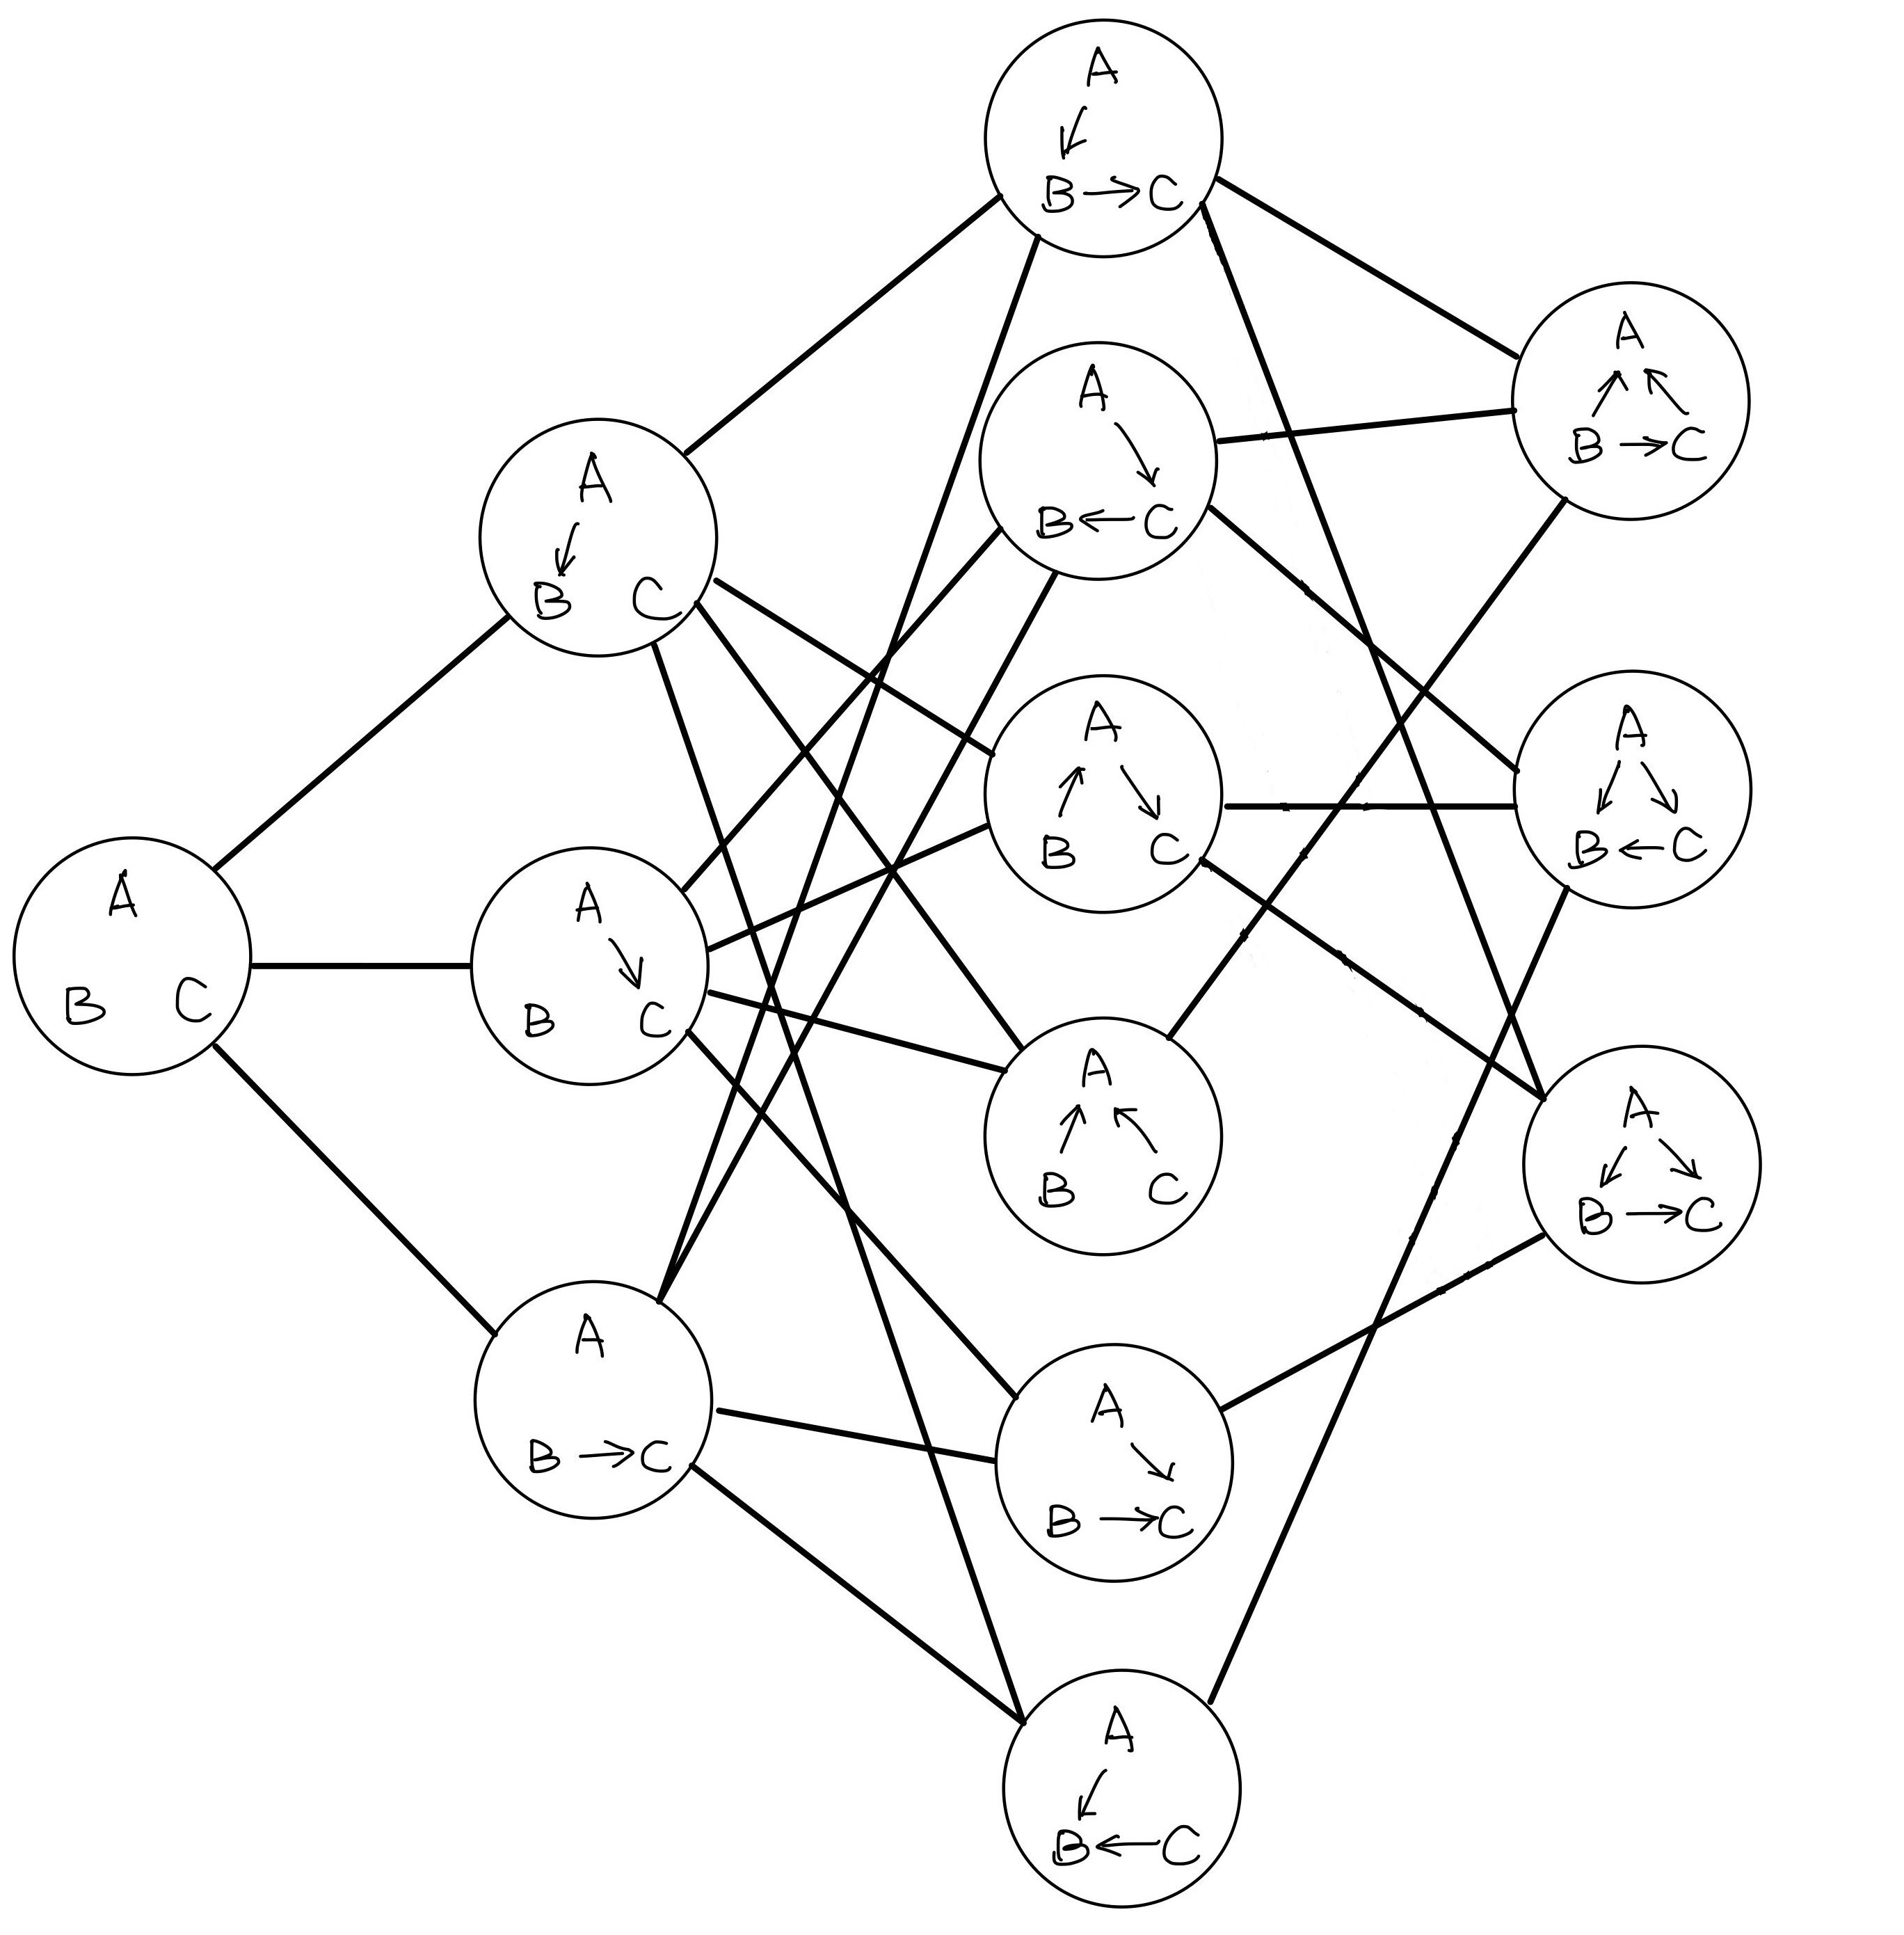
\includegraphics[scale=0.12]{graph}
\item[(d)]
There are two possible sequences.
\begin{enumerate}
\item[(1)]
$\{A\ B\ C\} \to \{A \to B, C; B \to A, C\} \to \{A \to B \to C; B \to A, B \to C; C \to B \to A\} \to \{A \to B \to C, A \to C; B \to A \to C, B \to C\} \to \{B \to A \to C; A \to B, A \to C; C \to A \to B\}$
\item[(2)]
$\{A\ B\ C\} \to \{A \to B, C; B \to A, C\} \to \{A \to B \to C; B \to A, B \to C; C \to B \to A\} \to \{A \to B \to C \to A; A \to C \to B \to A\} \to \{B \to A \to C; A \to B, A \to C; C \to A \to B\}$
\end{enumerate}
\item[(e)]
We should find equivalent DAGs with the following rules:
\begin{enumerate}
\item[(1)] Only reverse the direction of existing edges.
\item[(2)] Since there is no collider in the original DAG, there should also be no collider in the new DAG.
\end{enumerate}
Thus we have the following four equivalent DAGs: \\
$V_{1} \leftarrow V_{2} \to V_{3} \to V_{4} \to V_{5}$ \\
$V_{1} \leftarrow V_{2} \leftarrow V_{3} \to V_{4} \to V_{5}$ \\
$V_{1} \leftarrow V_{2} \leftarrow V_{3} \leftarrow V_{4} \to V_{5}$ \\
$V_{1} \leftarrow V_{2} \leftarrow V_{3} \leftarrow V_{4} \leftarrow V_{5}$ \\
\end{enumerate}
\end{answertext}

\newpage % for more space

\section*{Missing Data}

{\bf Question 2.}

\begin{enumerate}
\item[(a)] Consider the following observed data likelihood:
{\small
\begin{align*}
{\cal L}_{[D]}(\vec{\beta}) =& \prod_{i=1}^n \sum_{x^{(1)}_{2i} \text{ if }r_{2i}=0} \sum_{x^{(1)}_{4i} \text{ if }r_{4i}=0}  p(x_{1i}, x_{3i}) p(r_{4i} \mid x_{1i}, x_{3i}) p(r_{2i} \mid x_{1i})
p(x^{(1)}_{2i} \mid x_{1i})
p(x^{(1)}_{4i} \mid x_{3i}) \\
& 
p(x_{2i} \mid r_{2i}, x^{(1)}_{2i})
p(x_{4i} \mid r_{4i}, x^{(1)}_{4i})
\end{align*}
}
Draw the missing data graph for this model.
\item[(b)] Does this likelihood represent a missing at random (MAR) model or missing not at random (MNAR) model?
\item[(c)] Express $p(x_1, x_2^{(1)}, x_3, x_4^{(1)})$ as a function $p(x_1, x_2, x_3, x_4, r_2, r_4)$.
\item[(d)] Consider the following observed data likelihood:
{\small
\begin{align*}
{\cal L}_{[D]}(\vec{\beta}) =&
\prod_{i=1}^n
\sum_{x^{(1)}_{1i} \text{ if }r_{1i}=0}
\sum_{x^{(1)}_{2i} \text{ if }r_{2i}=0}
\sum_{x^{(1)}_{3i} \text{ if }r_{3i}=0}
p(x^{(1)}_{1i}) p(x^{(1)}_{2i} \mid x^{(1)}_{1i})
p(x^{(1)}_{3i} \mid x^{(1)}_{2i}, x^{(1)}_{1i})\\
& 
p(r_{1i} \mid x^{(1)}_{2i}, x^{(1)}_{3i})
p(r_{2i} \mid x^{(1)}_{1i}, r_{3i})
p(r_{3i} \mid x^{(1)}_{2i}, r_{1i})
\\
&
p(x_{1i} \mid r_{1i}, x^{(1)}_{1i})
p(x_{2i} \mid r_{2i}, x^{(1)}_{2i})
p(x_{3i} \mid r_{3i}, x^{(1)}_{3i})
\end{align*}
}
Draw the missing data graph for this model.
\item[(e)] Does this likelihood represent a missing at random (MAR) model or missing not at random (MNAR) model?
\item[(f)] Does the observed data likelihood have a unique global maximum?  In other words, 
 is $p(x_1^{(1)}, x_2^{(1)}, x_3^{(1)}, r_1, r_2, r_3)$ a function of the observed data distribution $p(x_1, x_2, x_3, r_1, r_2, r_3)$?  Why?  (This is a yes/no question with an explanation: if such a function exists, you don't have to give it)
\end{enumerate}

\begin{answertext}{22cm}{}
\begin{enumerate}
\item[(a)]The missing data graph is:\\
\begin{center}
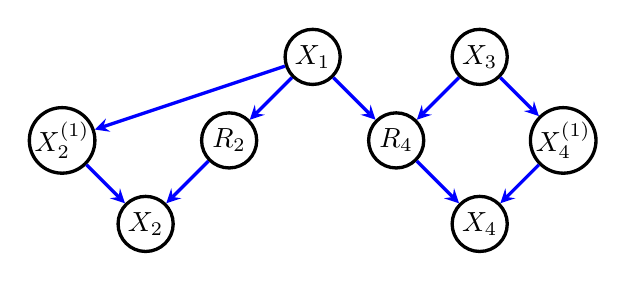
\begin{tikzpicture}[>=stealth, node distance=1.5cm]
    \tikzstyle{format} = [draw, very thick, circle, minimum size=7.0mm,
	inner sep=0pt]

		\path[->, very thick]
			node[format] (1) {$X_1$}
			node[format, below right of=1] (2) {$R_4$}
			node[format, below left of=1] (4) {$R_2$}
			node[format, below left of=4] (3) {$X_2$}
			node[format, above left of=3] (5) {$X_2^{(1)}$}
			node[format, below right of=2] (6) {$X_4$}
			node[format, above right of=2] (7) {$X_3$}
			node[format, below right of=7] (8) {$X_4^{(1)}$}

			(1) edge[blue] (2)
			(1) edge[blue] (4)
			(1) edge[blue] (5)
			(7) edge[blue] (2)
			(7) edge[blue] (8)
			(5) edge[blue] (3)
			(4) edge[blue] (3)
			(2) edge[blue] (6)
			(8) edge[blue] (6)
		;

\end{tikzpicture}
\end{center}
\item[(b)] This is a missing at random (MAR) problem. MAR means events that lead to missingness occur independently of unobserved data given observed data, and in this DAG we can clearly see $(X_2^{(1)} \ci R_2 \mid X_1)$ ($X_1$ fully observed) and $(X_4^{(1)} \ci R_4 \mid X_3)$ ($X_3$ fully observed). Thus, we fit the definition of MAR.

\item[(c)]
\begin{align*}
p(x_1, x_2^{(1)}, x_3, x_4^{(1)}) =& p(x_1, x_3)p(x_2^{(1)} \mid x_1)p(x_4^{(1)} \mid x_3)\\
=& p(x_1,x_3)p(x_2^{(1)} \mid x_1, r_2=1)p(x_4^{(1)} \mid x_3, r4=1)\\
=& p(x_1,x_3)p(x_2 \mid x_1, r_2=1)p(x_4 \mid x_3, r4=1)\\
=& \sum_{x_2,x_4,r_2,r_4}p(x_1, x_2, x_3, x_4, r_2, r_4)\\
& \cdot \frac{p(x_1, x_2, r_2=1)}{\sum_{x_2}p(x_1, x_2, r_2=1)}\\
& \cdot \frac{p(x_3, x_4, r_4=1)}{\sum_{x_4}p(x_3, x_4, r_4=1)}\\
=& \sum_{x_2,x_4,r_2,r_4}p(x_1, x_2, x_3, x_4, r_2, r_4)\\
& \cdot \frac{\sum_{x_3,x_4,r_4}p(x_1, x_2, x_3, x_4, r_2=1, r_4)}{\sum_{x_2}\sum_{x_3,x_4,r_4}p(x_1, x_2, x_3, x_4, r_2=1, r_4)}\\
& \cdot \frac{\sum_{x_1,x_2,r_2}p(x_1, x_2, x_3, x_4, r_2, r_4=1)}{\sum_{x_4}\sum_{x_1,x_2,r_2}p(x_1, x_2, x_3, x_4, r_2, r_4=1)}\\
=& \sum_{x_2,x_4,r_2,r_4}p(x_1, x_2, x_3, x_4, r_2, r_4)\\
& \cdot \frac{\sum_{x_3,x_4,r_4\text{ if }r_2=1}p(x_1, x_2, x_3, x_4, r_2, r_4)}{\sum_{x_2, x_3,x_4,r_4\text{ if }r_2=1}p(x_1, x_2, x_3, x_4, r_2, r_4)}\\
& \cdot \frac{\sum_{x_1,x_2,r_2\text{ if }r_4=1}p(x_1, x_2, x_3, x_4, r_2, r_4)}{\sum_{x_1,x_2,x_4,r_2\text{ if }r_4=1}p(x_1, x_2, x_3, x_4, r_2, r_4)}\\
\end{align*}

\end{enumerate}
\end{answertext} 

\begin{answertext}{22cm}{}
\begin{enumerate}
\item[(d)]The missing data graph is:\\
\begin{center}
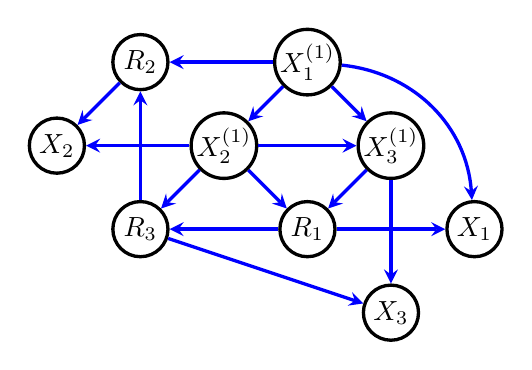
\begin{tikzpicture}[>=stealth, node distance=1.5cm]
    \tikzstyle{format} = [draw, very thick, circle, minimum size=7.0mm,
	inner sep=0pt]

		\path[->, very thick]
			node[format] (1) {$X_1^{(1)}$}
			node[format, below right of=1] (2) {$X_3^{(1)}$}
			node[format, below left of=1] (4) {$X_2^{(1)}$}
			node[format, below left of=4] (3) {$R_3$}
			node[format, above left of=3] (5) {$X_2$}
			node[format, below right of=2] (6) {$X_1$}
			node[format, below left of=2] (7) {$R_1$}
			node[format, below right of=7] (8) {$X_3$}
			node[format, above right of=5] (9) {$R_2$}

			(1) edge[blue] (2)
			(1) edge[blue] (4)
			(4) edge[blue] (2)
			(4) edge[blue] (7)
			(2) edge[blue] (7)
			(4) edge[blue] (3)
			(7) edge[blue] (3)
			(1) edge[blue] (9)
			(3) edge[blue] (9)
			(9) edge[blue] (5)
			(4) edge[blue] (5)
			(2) edge[blue] (8)
			(3) edge[blue] (8)
			(1) edge[blue,bend left=40] (6)
			(7) edge[blue] (6)
		;

\end{tikzpicture}
\end{center}

\item[(e)]This is a missing not at random (MNAR) model. As none of the X are completely known, we can see that $X_1^{(1)}$ and $R_1$ are not independent because we don't know $X_2^{(1)}$; $X_2^{(1)}$ and $R_2$ are not independent because we don't know $X_1^{(1)}$; $X_3^{(1)}$ and $R_3$ are not independent because we don't know $X_1^{(1)}$ and $X_2^{(1)}$. Clearly, this is missing not at random because the missingness and unobserved data are clearly dependent.

\item[(f)]no, it does not. we know that all missingness and unobserved data are dependent, so there is no way we can bring $R_i=1$ condition into the factorization and replace $X_i^{(1)}$ with $X_i$. Thus, it is not possible write $p(x_1^{(1)}, x_2^{(1)}, x_3^{(1)}, r_1, r_2, r_3)$ as a function of the observed data distribution $p(x_1, x_2, x_3, r_1, r_2, r_3)$.

\end{enumerate}
\end{answertext} 

\pagebreak

\section*{PCA.}

\begin{enumerate}
\item[(a)] Assume we performed PCA on a centered dataset $[D^*]$ of size $n$ by $k$, and kept the first $m$ eigenvalues of the sample covariance matrix $\hat{C}$.
In other words, the new dataset $[\tilde{D}] = [D^*] [V]_m$ is a matrix of size $n$ by $m$, where $[V]_m$ is a $k$ by $m$ matrix containing the $m$ eigenvectors corresponding to the largest eigenvalues
of $\hat{C}$.  Let $i$ and $j$ be different column indices in $[V]_m$.  Show that the sample covariance between the corresponding columns of $[\tilde{D}]$ is $0$ (meaning that the $i$th and $j$th features in $[\tilde{D}]$ are uncorrelated.

Hints: the sample covariance of any dataset $[X]$ is proportional to $[X]^T [X]$.  You may use the fact that eigenvectors are all orthogonal to each other, meaning that if $\vec{v}_i$, $\vec{v}_j$ are eigenvectors, then $\vec{v}_i \vec{v}_j = 0$.  Finally, note that given a matrix $[A]$, and its eigenvalue $\lambda_i$, and the corresponding eigenvector $\vec{v}_i$, $[A] \vec{v}_i = \lambda \vec{v}_i$.

\item[(b)] PCA is a dimension reduction method that aims to find a $k$-dimensional description of $m$-dimensional data (where $k$ is hopefully much smaller than $m$).
Kernel PCA aims to project $m$ into a very high dimensional (possibly infinite dimensional) space using a kernel $K(x_i,x_j)$.  Given that the goal is to reduce dimension of the
original data $[D]$, what is the point of projecting to a high dimensional space prior to reducing dimension to $k$?

\end{enumerate}

\begin{answertext}{14cm}{}
\begin{enumerate}
\item[(a)] We know that the sample covariance matrix of $[\tilde{D}]$ is proportional to $[\tilde{D}]^T [\tilde{D}]$, so we can first calculate $[\tilde{D}]^T [\tilde{D}]$, and if any element $a_{ij}$ is 0 in $[\tilde{D}]^T [\tilde{D}]$ , the covariance of $i$ and $j$ column in $[\tilde{D}]$ should also be 0.
\begin{align*}
[\tilde{D}]^T [\tilde{D}] &= ([D^*] [V]_m)^T[D^*] [V]_m\\
&= [V]_m^T [D^*]^T [D^*] [V]_m
\end{align*}
We know that $\hat{C} = \frac{1}{n-1}[D^*]^T [D^*]$, so we have $[D^*]^T [D^*]=(n-1)\hat{C}$. Plug it in:
\begin{align*}
[\tilde{D}]^T [\tilde{D}] &= [V]_m^T [D^*]^T [D^*] [V]_m\\
&= [V]_m^T (n-1)\hat{C} [V]_m\\
&= (n-1) [V]_m^T \hat{C} [V]_m\\
&= (n-1)
\begin{bmatrix}
\vec{v}_1^T\\
\vec{v}_2^T\\
\vdots\\
\vec{v}_m^T
\end{bmatrix}
\hat{C}
\begin{bmatrix}
\vec{v}_1 & \vec{v}_2 & \cdots & \vec{v}_m
\end{bmatrix}\\
&= (n-1)
\begin{bmatrix}
\vec{v}_1^T\\
\vec{v}_2^T\\
\vdots\\
\vec{v}_m^T
\end{bmatrix}
\begin{bmatrix}
\hat{C}\vec{v}_1 & \hat{C}\vec{v}_2 & \cdots & \hat{C}\vec{v}_m
\end{bmatrix}
\end{align*}
As $\vec{v}_i$ is eigenvector of $\hat{C}$, we have $\hat{C}\vec{v}_i = \lambda_i \vec{v}_i$:
\end{enumerate}
\end{answertext}

\begin{answertext}{22cm}{}
\begin{align*}
[\tilde{D}]^T [\tilde{D}] &= (n-1)
\begin{bmatrix}
\vec{v}_1^T\\
\vec{v}_2^T\\
\vdots\\
\vec{v}_m^T
\end{bmatrix}
\begin{bmatrix}
\hat{C}\vec{v}_1 & \hat{C}\vec{v}_2 & \cdots & \hat{C}\vec{v}_m
\end{bmatrix}\\
&=(n-1)
\begin{bmatrix}
\vec{v}_1^T\\
\vec{v}_2^T\\
\vdots\\
\vec{v}_m^T
\end{bmatrix}
\begin{bmatrix}
\lambda_1\vec{v}_1 & \lambda_2\vec{v}_2 & \cdots & \lambda_m\vec{v}_m
\end{bmatrix}\\
&=(n-1)
\begin{bmatrix}
\lambda_1 \vec{v}_1^T \vec{v}_1 & \lambda_2 \vec{v}_1^T \vec{v}_2 & \cdots & \lambda_m \vec{v}_1^T \vec{v}_m\\
\lambda_1 \vec{v}_2^T \vec{v}_1 & \lambda_2 \vec{v}_2^T \vec{v}_2 & \cdots & \lambda_m \vec{v}_2^T \vec{v}_m\\
\vdots & \vdots & \ddots & \vdots\\
\lambda_1 \vec{v}_m^T \vec{v}_1 & \lambda_2 \vec{v}_m^T \vec{v}_2 & \cdots & \lambda_m \vec{v}_m^T \vec{v}_m
\end{bmatrix}
\end{align*}
We know that eigenvectors are all orthogonal to each other, so $\vec{v}_i^T \vec{v}_j=0$ when $i \neq j$. Then to covariance matrix becomes:
\begin{align*}
[\tilde{D}]^T [\tilde{D}] &=(n-1)
\begin{bmatrix}
\lambda_1 \vec{v}_1^T \vec{v}_1 & \lambda_2 \vec{v}_1^T \vec{v}_2 & \cdots & \lambda_m \vec{v}_1^T \vec{v}_m\\
\lambda_1 \vec{v}_2^T \vec{v}_1 & \lambda_2 \vec{v}_2^T \vec{v}_2 & \cdots & \lambda_m \vec{v}_2^T \vec{v}_m\\
\vdots & \vdots & \ddots & \vdots\\
\lambda_1 \vec{v}_m^T \vec{v}_1 & \lambda_2 \vec{v}_m^T \vec{v}_2 & \cdots & \lambda_m \vec{v}_m^T \vec{v}_m
\end{bmatrix}\\
&= (n-1)
\begin{bmatrix}
\lambda_1 \vec{v}_1^T \vec{v}_1 & 0 & \cdots & 0\\
0 & \lambda_2 \vec{v}_2^T \vec{v}_2 & \cdots & 0\\
\vdots & \vdots & \ddots & \vdots\\
0 & 0 & \cdots & \lambda_m \vec{v}_m^T \vec{v}_m
\end{bmatrix}
\end{align*}
We can see that except for the main diagonal elements which are proportional to the sample covariance between the same column and itself in $[\tilde{D}]$, all other elements are zero. The zeros in covariances matrix of $[\tilde{D}]$ show that any two different columns of $[\tilde{D}]$ has covariance zero. This means that for all different columns in $[V]_m$, the sample covariance between the corresponding columns of $[\tilde{D}]$
are zero, as there is one-to-one correspondence between columns in $[V]_m$ and $[\tilde{D}]$. 
\end{answertext}
\begin{answertext}{14cm}{}
\begin{enumerate}
\item[(b)] There are several reasons and benefits for using kernel PCA. First, PCA itself is a linear transformation, and each principal component is a linear combination of the original data point. That means when doing PCA, we are actually assuming linearity in the data, and are trying to use linear transformation to map the data into lower dimensions with largest variance. However, for many datasets, especially the high-dimensional data, it is not possible to find a lower dimensional space using linear transformation that can separate the data well (i.e. find eigenvector with large variance associated with it). In this case, the separation of data is non-linear, and we would need a non-linear transformation to map the data into a better low-dimensional space with larger variance in each axis. This is why we need a kernel here. The kernel trick first use a non-linear transformation to transform the data into a much higher dimensional space, and then finding eigenvector there can give you a larger variance and better separation of data in the resulting low-dimensional space. Second, even if we have transformed the data to a higher dimensional space and reduced it again, the non-linear transformation we added through this process will likely to cause the data to lie on a lower dimensional subspace of it. Thus, we increased the dimension first in order to be able to better decrease it into a lower dimensional space with higher variance and better separation of data.
\end{enumerate}
\end{answertext}

\pagebreak

% -----------------------------------------------------------

\end{document}
